\begin{figure}[!htbp]
\centering
\resizebox{\linewidth}{!}{%
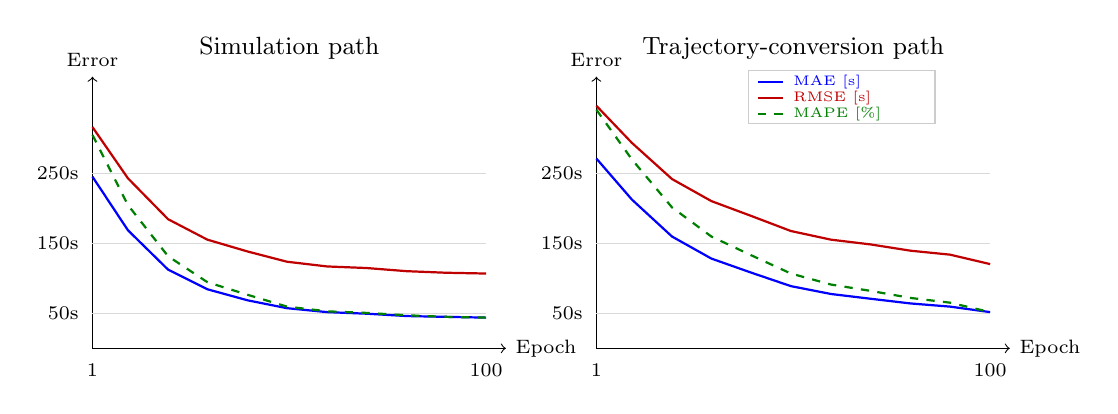
\begin{tikzpicture}

\begin{scope}[xshift=0cm]
  \draw[->] (0.8,0.7) -- (6.05,0.7) node[right] {\scriptsize Epoch};
  \draw[->] (0.8,0.7) -- (0.8,4.15) node[above] {\scriptsize Error};
  \draw[gray!30] (0.8,1.14) -- (5.8,1.14);
  \draw[gray!30] (0.8,2.03) -- (5.8,2.03);
  \draw[gray!30] (0.8,2.92) -- (5.8,2.92);
  \node[anchor=south] at (3.30,4.25) {\small Simulation path};
  \draw[blue, thick] (0.80,2.88) -- (1.25,2.20) -- (1.76,1.70) -- (2.26,1.45) -- (2.77,1.31) -- (3.27,1.21) -- (3.78,1.16) -- (4.28,1.14) -- (4.79,1.11) -- (5.29,1.10) -- (5.80,1.09);
  \draw[red!75!black, thick] (0.80,3.51) -- (1.25,2.86) -- (1.76,2.34) -- (2.26,2.08) -- (2.77,1.93) -- (3.27,1.80) -- (3.78,1.74) -- (4.28,1.72) -- (4.79,1.68) -- (5.29,1.66) -- (5.80,1.65);
  \draw[green!50!black, thick, dashed] (0.80,3.41) -- (1.25,2.52) -- (1.76,1.87) -- (2.26,1.54) -- (2.77,1.38) -- (3.27,1.23) -- (3.78,1.17) -- (4.28,1.15) -- (4.79,1.12) -- (5.29,1.10) -- (5.80,1.09);
  \node[anchor=north] at (0.8,0.62) {\scriptsize 1};
  \node[anchor=north] at (5.80,0.62) {\scriptsize 100};
  \node[anchor=east] at (0.75,1.14) {\scriptsize 50s};
  \node[anchor=east] at (0.75,2.03) {\scriptsize 150s};
  \node[anchor=east] at (0.75,2.92) {\scriptsize 250s};
\end{scope}


\begin{scope}[xshift=6.4cm]
  \draw[->] (0.8,0.7) -- (6.05,0.7) node[right] {\scriptsize Epoch};
  \draw[->] (0.8,0.7) -- (0.8,4.15) node[above] {\scriptsize Error};
  \draw[gray!30] (0.8,1.14) -- (5.8,1.14);
  \draw[gray!30] (0.8,2.03) -- (5.8,2.03);
  \draw[gray!30] (0.8,2.92) -- (5.8,2.92);
  \node[anchor=south] at (3.30,4.25) {\small Trajectory-conversion path};
  \draw[blue, thick] (0.80,3.11) -- (1.25,2.59) -- (1.76,2.12) -- (2.26,1.84) -- (2.77,1.66) -- (3.27,1.49) -- (3.78,1.39) -- (4.28,1.33) -- (4.79,1.27) -- (5.29,1.23) -- (5.80,1.16);
  \draw[red!75!black, thick] (0.80,3.78) -- (1.25,3.31) -- (1.76,2.85) -- (2.26,2.57) -- (2.77,2.38) -- (3.27,2.19) -- (3.78,2.08) -- (4.28,2.02) -- (4.79,1.94) -- (5.29,1.89) -- (5.80,1.77);
  \draw[green!50!black, thick, dashed] (0.80,3.73) -- (1.25,3.10) -- (1.76,2.49) -- (2.26,2.12) -- (2.77,1.88) -- (3.27,1.65) -- (3.78,1.51) -- (4.28,1.43) -- (4.79,1.34) -- (5.29,1.28) -- (5.80,1.16);
  \node[anchor=north] at (0.8,0.62) {\scriptsize 1};
  \node[anchor=north] at (5.80,0.62) {\scriptsize 100};
  \node[anchor=east] at (0.75,1.14) {\scriptsize 50s};
  \node[anchor=east] at (0.75,2.03) {\scriptsize 150s};
  \node[anchor=east] at (0.75,2.92) {\scriptsize 250s};
\end{scope}

\begin{scope}[shift={(9.25,3.65)}]
  \draw[fill=white, draw=gray!40] (-0.12,-0.10) rectangle (2.25,0.58);
  \draw[blue, thick] (0,0.43) -- (0.32,0.43) node[right] {\tiny MAE [s]};
  \draw[red!75!black, thick] (0,0.23) -- (0.32,0.23) node[right] {\tiny RMSE [s]};
  \draw[green!50!black, thick, dashed] (0,0.03) -- (0.32,0.03) node[right, align=left] {\tiny MAPE [\%]};
\end{scope}
\end{tikzpicture}
}
\caption[Representative 100-epoch validation curves for both construction paths.]{Representative 100-epoch validation curves for the two construction paths. Both curves converge, while the trajectory-conversion path converges later because its active-traffic snapshots are sparser; the denser simulation snapshots expose dynamic vehicle and relation edges more frequently during training.}
\label{fig:training_curves}
\end{figure}
